
\section{Durchführung}
\label{sec:Durchführung}

\subsection{Material}
Bei diesem Versuch wird ein Diodenlaser nach dem Littrow-Aufbau verwendet. 
Mit Hilfe eines sechskantigen Winkelschraubendrehers, kann das Beugungsgitter verstellt werden.
Das Gitter und die Kollimationslinse sind fest im Laser verbaut, der wiederum auf einem optischen Tisch befestigt ist.
Zudem werden eine CCD-Kammera und eine Detektorkarte verwendet, um den Infrarotlaser sichtbar zu machen.
Außerdem wird eine Rubidium-Zelle, zwei Photodioden, Linsen und Filter, so wie ein 50/50-Strahlteiler verwendet.
Während der Messungen wird der Laser auf eine Betriebstemperatur von $\SI{50}{\celsius}$ geheizt, um die für das Rubidium relevante Wellenlänge zu emittieren.
Zur Auswertung steht ein Oszilloskop zur verfügung.



\subsection{Schwellenstrom}
\label{sec:schwellenstrom}

Zu Beginn wird der Schwellenstrom bestimmt, ab dem von LED-Betrieb auf Laser-Betrieb gewechselt wird.
Dieser Schwellenwert wird durch Lasergranulation bestimmt.
Diese tritt auf, wenn starkes monochromatisches, kohärentes Licht auf eine unebene Oberfläche trifft.
Dabei müssen die Unebenheiten in der Größenordnung der Wellenlänge sein, damit nach dem Huygen'schen Prinzip das Licht gestreut wird.
Dadurch entstehen zufällige Interferenzmuster, was sich in einem körnigen Lichtfleck auf der Detektorkarte äußert.
Im LED-Bereich treten diese Interferenzmuster nicht auf, da das emittierte Licht nicht kohärent ist.

Um den Schwellenstrom zu ermitteln, wird der Aufbau gemäß Abbildung \ref{fig:th} aufgebaut.
Anschließend wird der Betriebsstrom schrittweise erhöht und kurz vor, so wie kurz nach erreichen des Schwellenstroms.
Danach werden langsam der Strom und der Winkel des Lasers verändert, bis der Strom den kleinst möglichen Wert angenommen hat.

\begin{figure}[H]
	\centering
	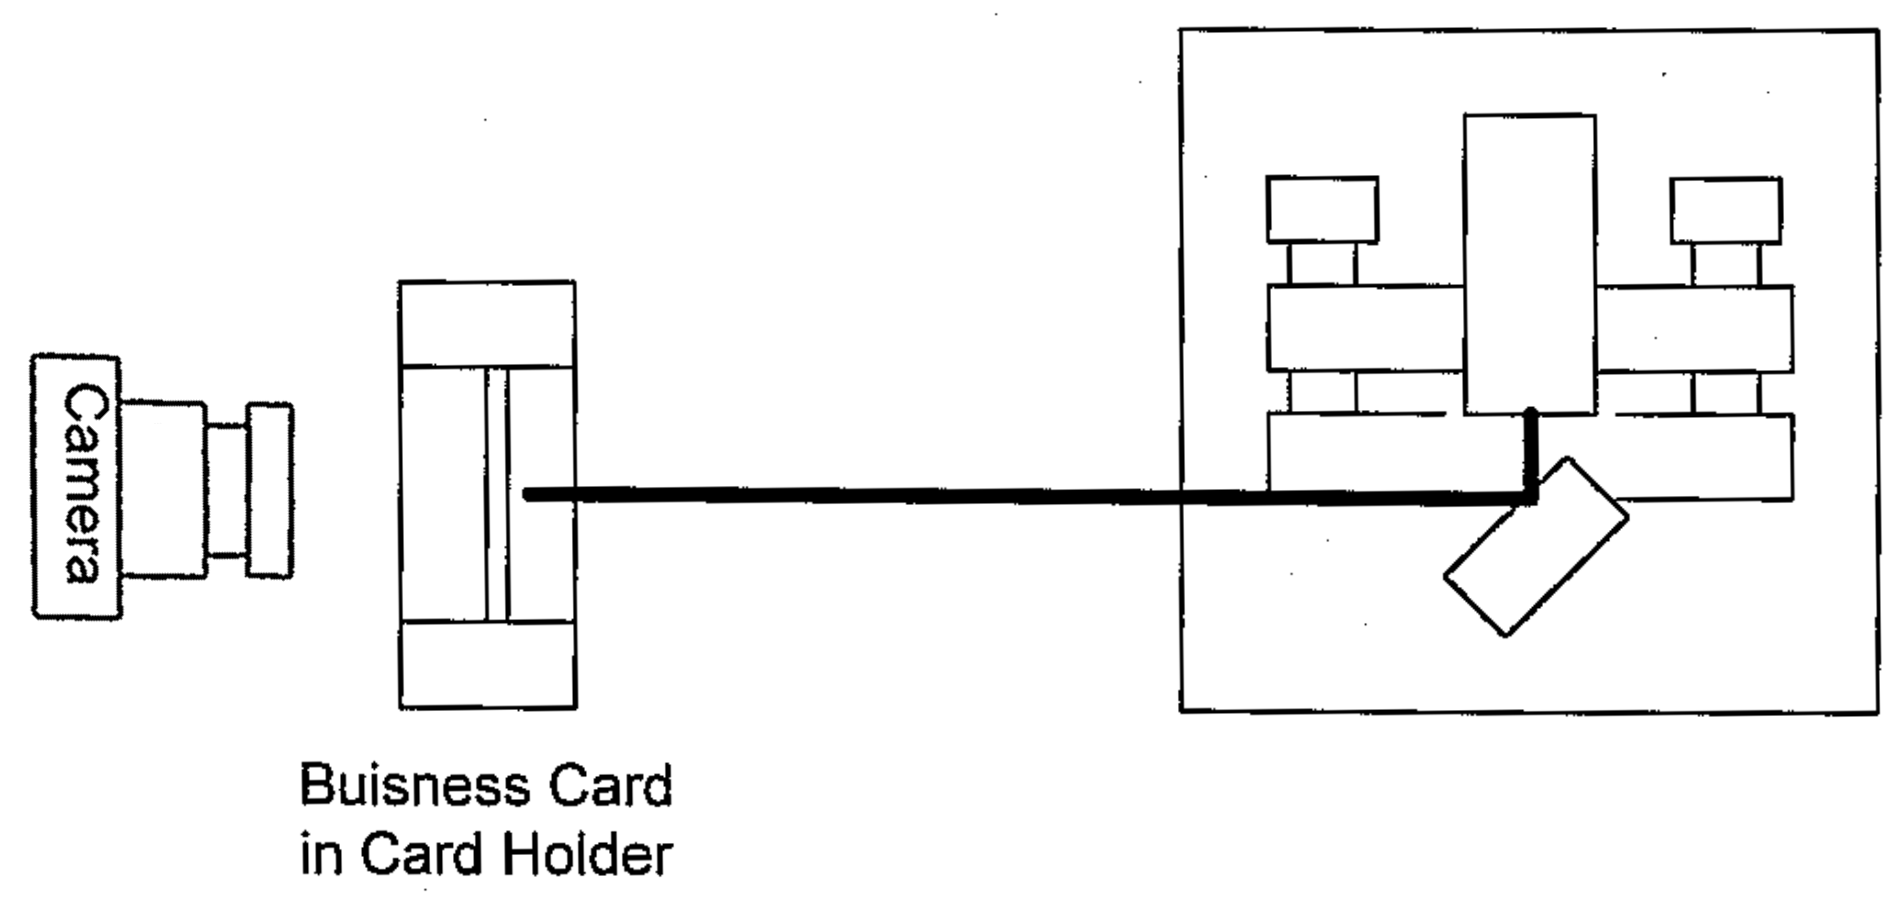
\includegraphics[width=\textwidth]{plots/setup_threshold.png}
	\caption{Aufbau um den Schwellstrom zu ermitteln. \cite{V60}}
	\label{fig:th}
\end{figure}

\subsection{Rubidiumfluoriszenz und Transmissionsspektrum}
\label{sec:Rubidium}

Für die Messung der Rubidiumfluoreszenz, wird der Aufbau gemäß Abbildung \ref{fig:sub} realisiert.
Damit der Laser stark genug ist, wird der Betriebsstrom deutlich über den Schwellenwert angesetzt.
Nun wird der Piezo-Kristall, das Gitter und der Strom fein justiert, bis die Rubidiumfluoriszenz auf der CCD-Kamera sichtbar wird.

Zur Aufnahme des Rubidium-Transmissionsspektrums, wird vor die Rubidium-Zelle ein 50/50-Teiler platziert.
Eine Hälfte des Strahls wird durch die Rubidium-Zelle gelenkt und anschließend auf eine Photodiode.
Die andere Hälfte wird direkt auf eine Photodiode gelenkt.
Um die Photodioden möglichst wenig zu stören wird bei dieses Messung das Raumlicht ausgeschaltet.
Beide Photodioden werden an einen Funktionsgenerator angeschlossen, mit dessen Hilfe die Differenz der beiden Strahlen gebildet wird und somit die Veränderung durch die Rubidium-Zelle.
Das Ergebnis wird durch ein Oszilloskop veranschaulicht.
Um Modensprünge zu verhindern, wird der Laser erneut wie im vorherigen Schritt justiert.


\begin{figure}[H]
	\centering
	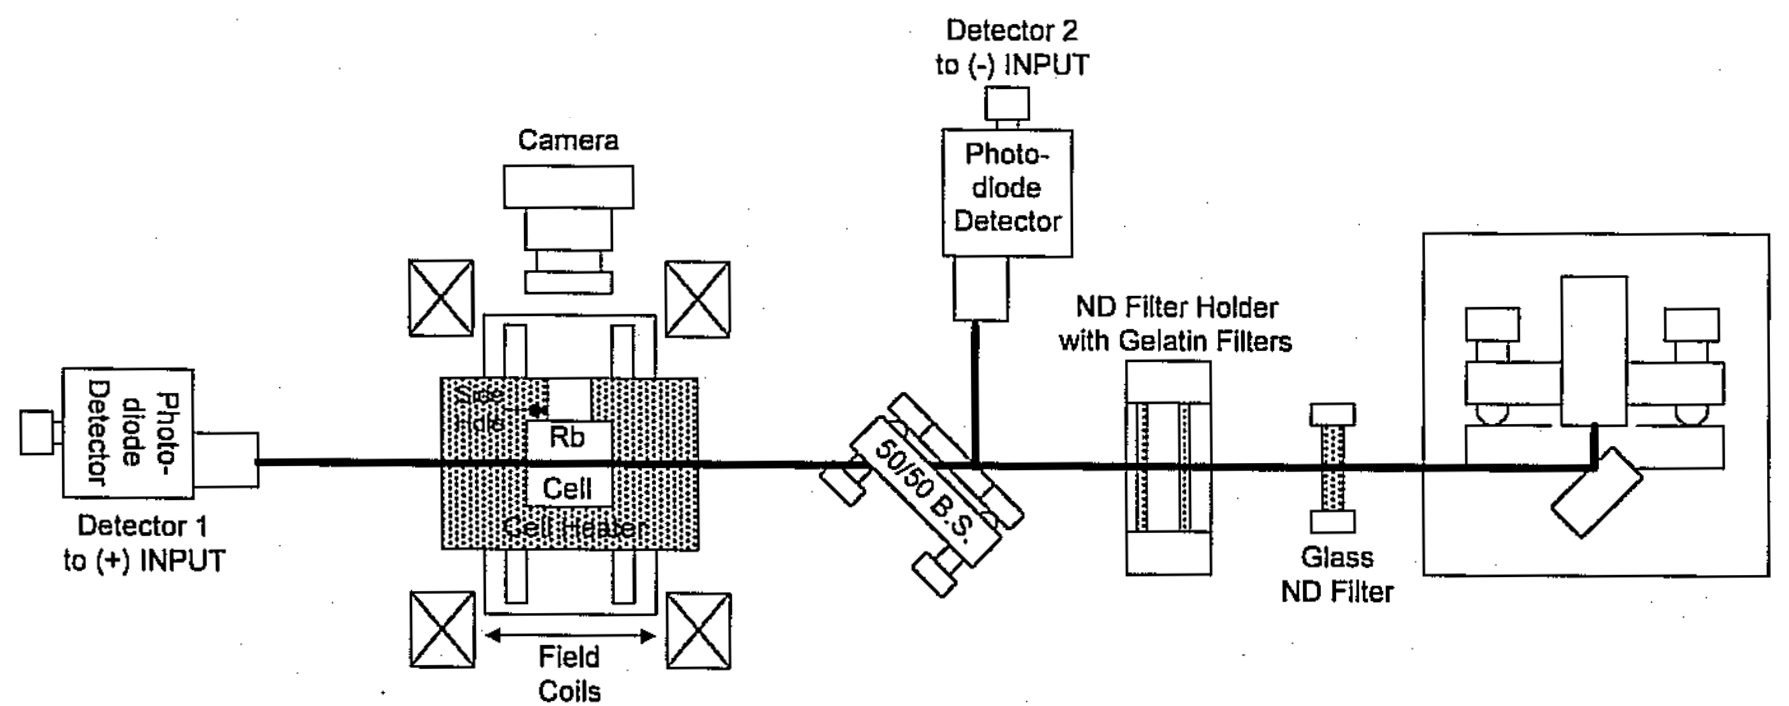
\includegraphics[width=\textwidth]{plots/setup_substraction.png}
	\caption{Aufbau, um die Rubidiumfluoreszenz zu messen. \cite{V60}}
	\label{fig:sub}
\end{figure}